\documentclass{article}
\usepackage[utf8]{inputenc}
\usepackage[spanish]{babel}
\usepackage{listings}
\usepackage{graphicx}
\graphicspath{ {images/} }
\usepackage{cite}


\begin{document}

\begin{titlepage}
    \begin{center}
        \vspace*{1cm}
            
        \Huge
        \textbf {Proyecto Final: Idea Final}
            
        \vspace{0.5cm}
        \LARGE
        Informatica II
            
        \vspace{1.5cm}
            
        \textbf{Daniela Andrea Gallego Díaz\\ Manuela Gutiérrez Rodríguez }
            
        \vfill
            
        \vspace{0.8cm}
            
        \Large
        Despartamento de Ingeniería Electrónica y Telecomunicaciones\\
        Universidad de Antioquia\\
        Medellín\\
        Septiembre de 2021
            
    \end{center}
\end{titlepage}

\tableofcontents
\newpage

\section{Idea Final: The Master Key} \label{contenido}

El juego consiste en un personaje que se desplaza a través de un laberinto mientras debe enfrentarse a sus enemigos, cuando derrote al indicado encontrará la llave maestra para abrir una puerta y subir de nivel.


\subsection{Menú principal}
En este se encontrará la opción de introducir un nombre de usuario, además de elegir entre las 3 opciones de niveles disponibles (fácil, intermedio, difícil).


Nota: al finalizar cada nivel se le preguntará al usuario si desea continuar el siguiente nivel (en el caso del nivel fácil e intermedio) o si desea salir al menú de inicio.

\begin{figure}[h!]
    \centering
    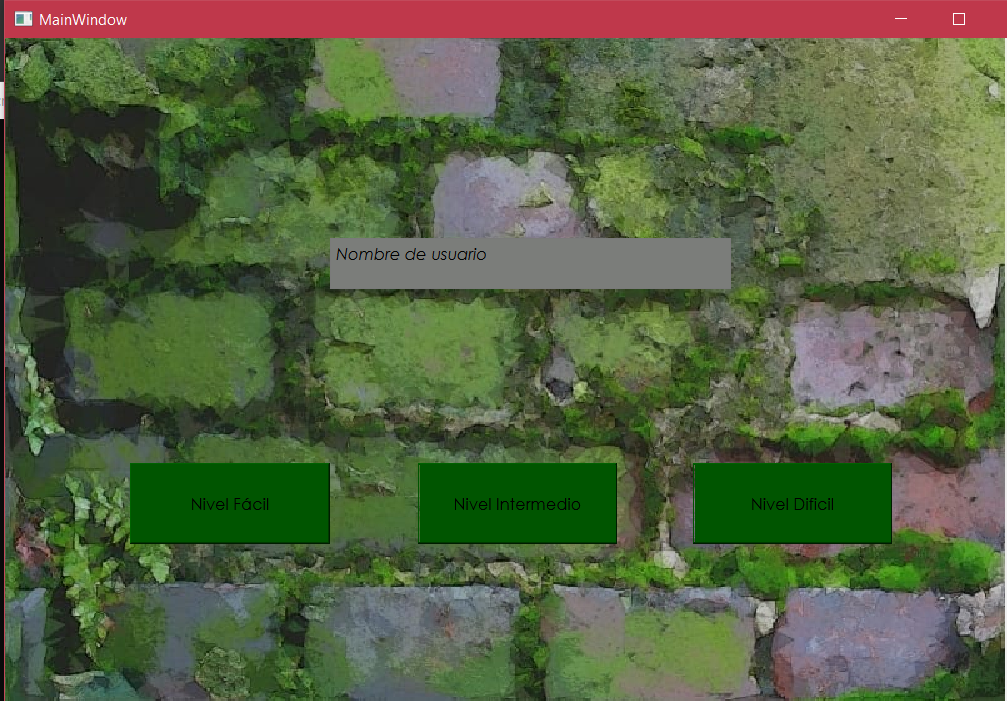
\includegraphics[scale=0.6]{muestra.png}
\end{figure}
 
\newpage

\subsection{Escenario}
Estará compuesto de laberintos que cambiarán de dificultad en cada nivel, al final de cada laberinto se encontrará con la puerta, si logra abrirla pasará al siguiente nivel.

\begin{itemize}
\item Nivel fácil: compuesto por un laberinto relativamente sencillo de realizar, dos enemigos a los cuales el personaje principal se debe enfrentar y una puerta de fácil acceso.
\item Nivel intermedio: compuesto por un laberinto de mayor nivel, con caminos sin salidas y tres enemigos con mayor dificultad de asesinar, acceder a la puerta es un poco más complicado.
\item Nivel difícil: compuesto por un mega laberinto, con diversos caminos sin salida y solo dos caminos posibles, los cuatro enemigos además de ser más complicados de asesinar incluirán la posibilidad de perseguir al personaje, la puerta tiene un acceso difícil. 
\end{itemize}

\begin{figure}[h!]
    \centering
    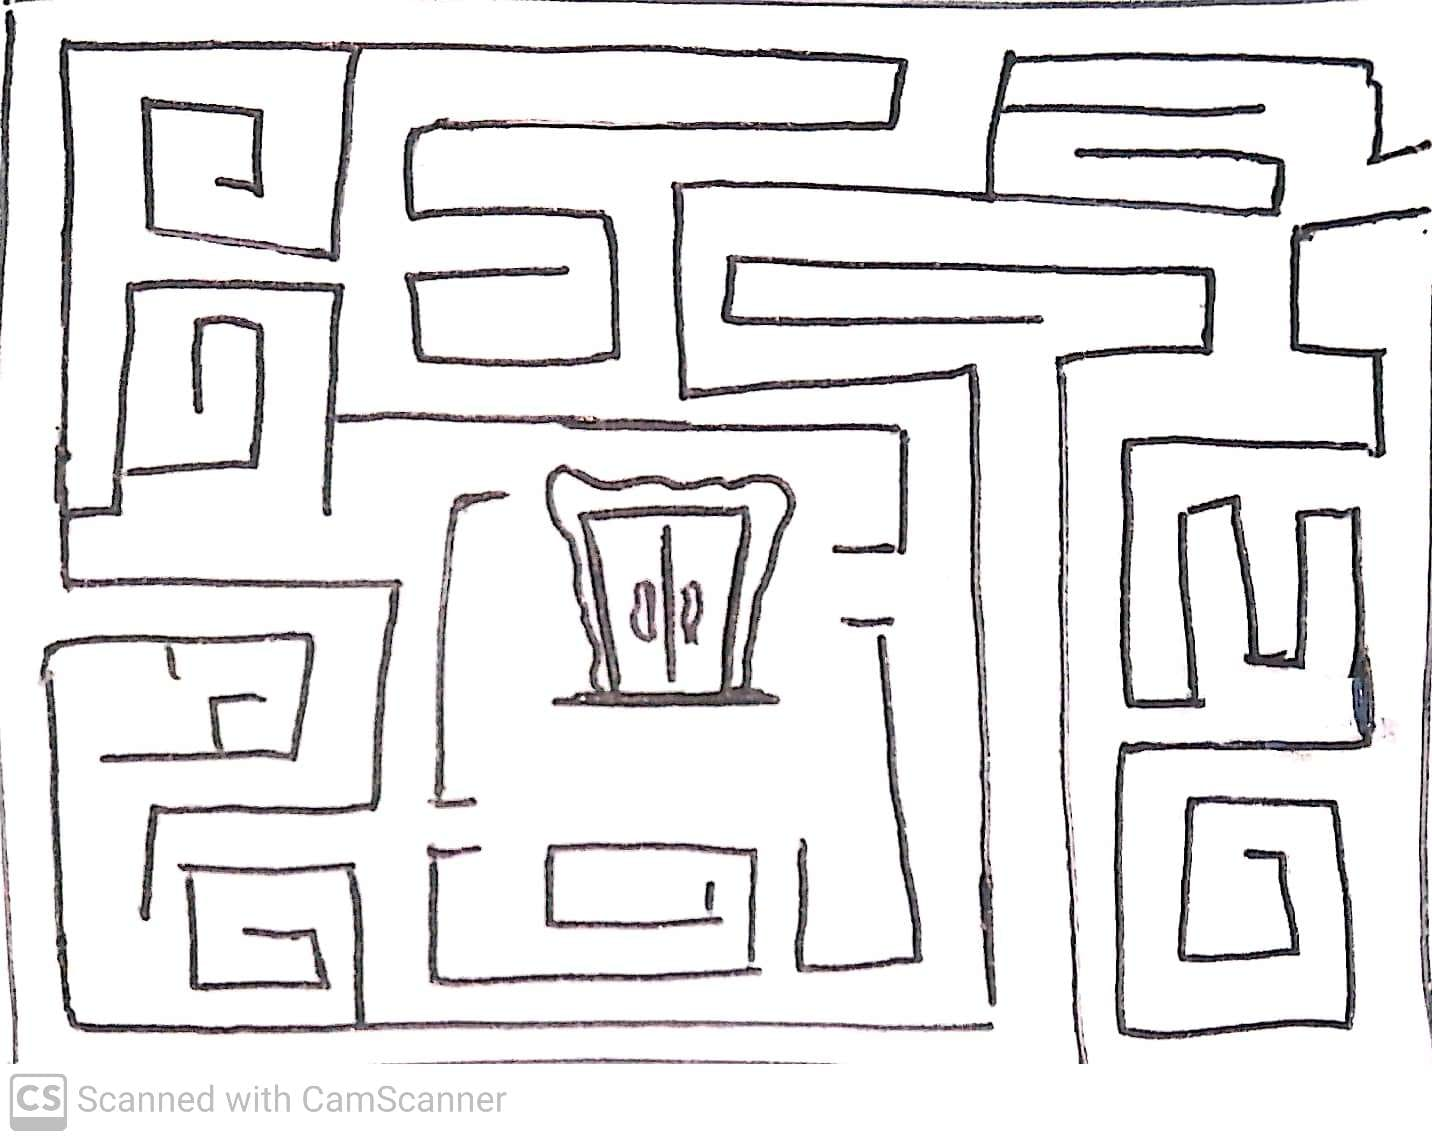
\includegraphics[scale=0.2]{WhatsApp Image 2021-09-14 at 12.02.29 PM.jpeg}
\end{figure}

\newpage

\subsection{Personaje principal}
Nuestro protagonista es Robin Hood, él deberá enfrentarse a cada enemigo para encontrar la llave, para ello deberá utilizar sus flechas e infringir daño a los contrincantes hasta asesinarlos, además de lograr pasar el laberinto y encontrar la puerta.


\begin{figure}[h!]
    \centering
    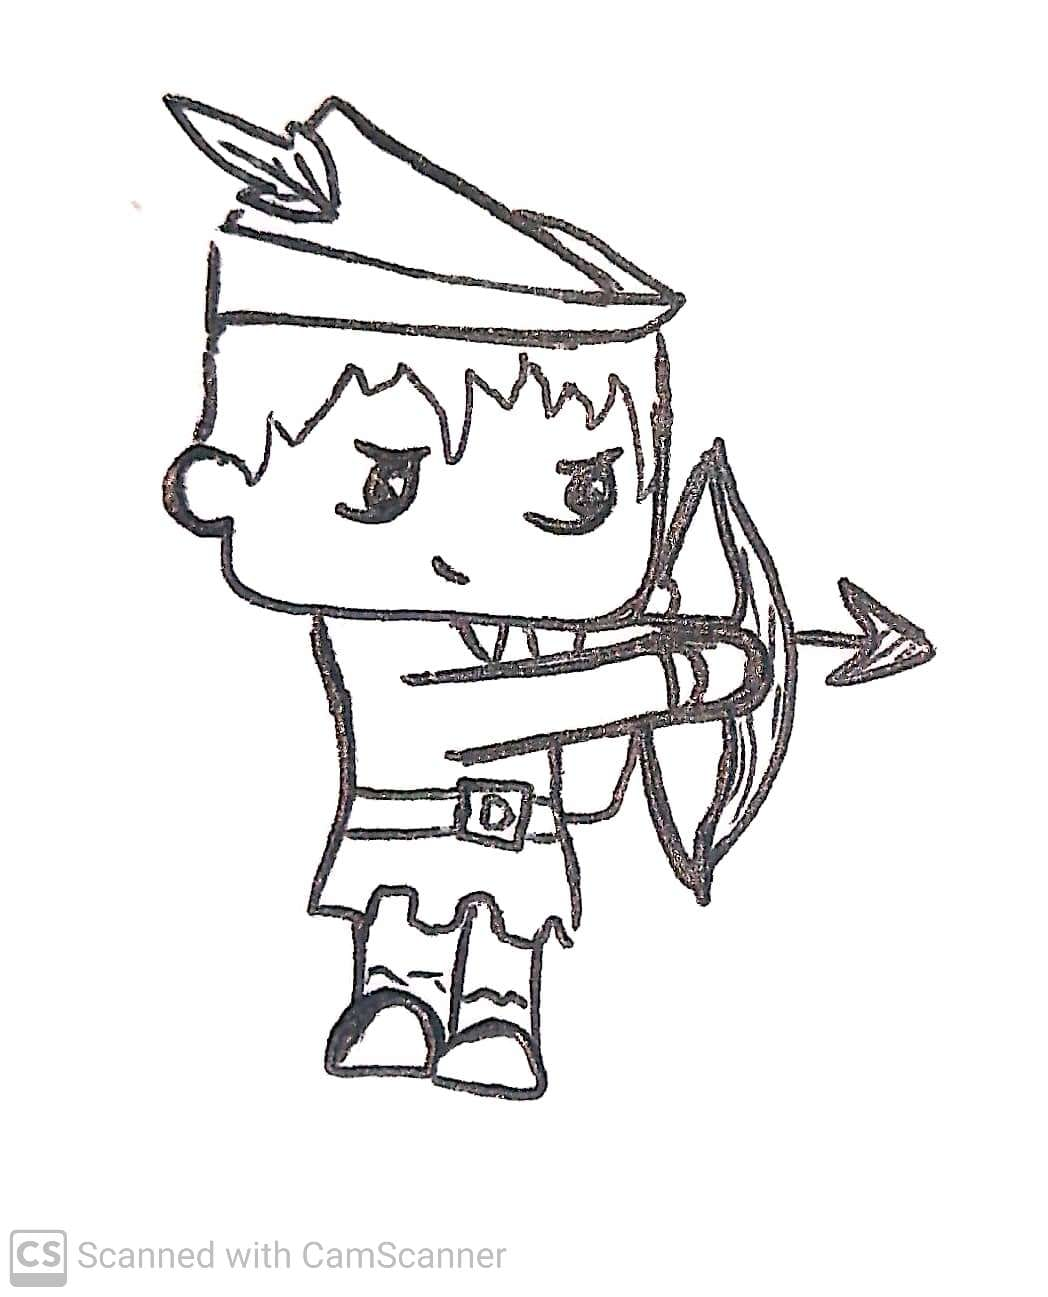
\includegraphics[scale=0.3]{WhatsApp Image 2021-09-14 at 12.01.50 PM.jpeg}
\end{figure}

\newpage


\subsection{Los enemigos}
Cada enemigo será más resistente a las flechas de Robin al subir de nivel, por lo que será más difícil derribarlos. Uno de ellos tiene en su poder la llave maestra y hará lo posible para no dejar que Robin se la lleve. Los enemigos aumentan cuando se sube de nivel, lo que hace más difícil la misión de conseguir la llave.

\begin{figure}[h!]
    \centering
    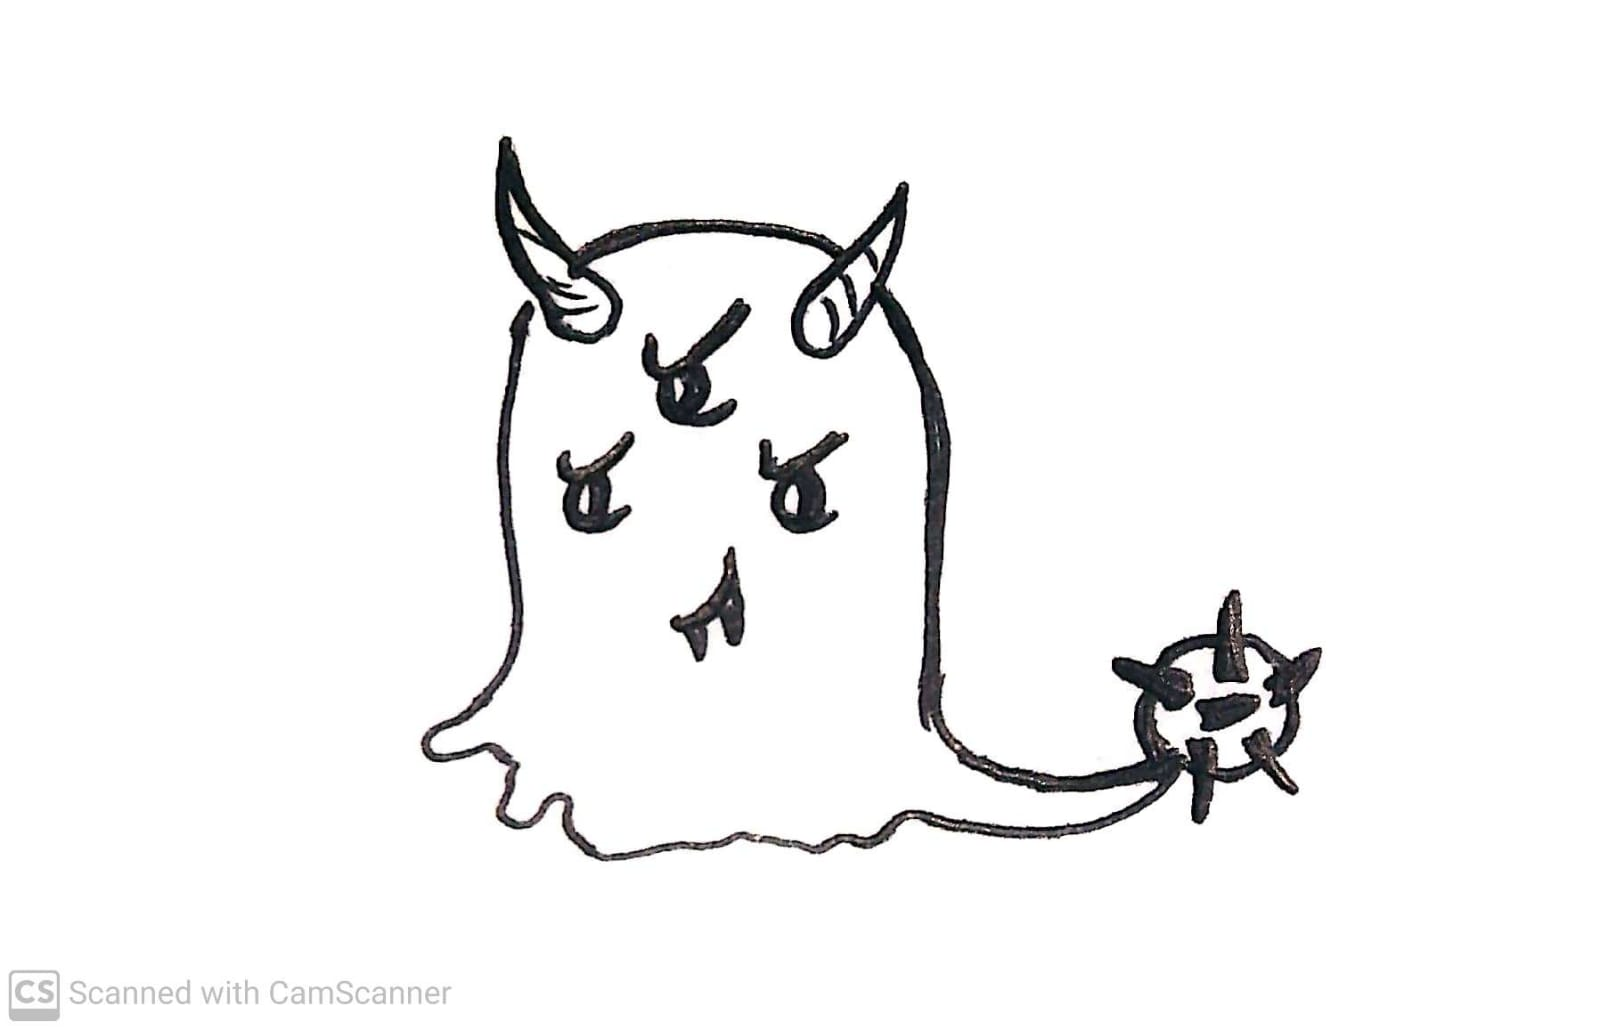
\includegraphics[scale=0.3]{WhatsApp Image 2021-09-14 at 12.02.08 PM.jpeg}
\end{figure}

\newpage


\subsection{La llave}
esta llave maestra aparecerá únicamente cuando se haya matado al enemigo indicado, por lo que el personaje debe asesinar a la cantidad de monstruos necesarios para acceder a esta, la puerta de salida no se abre a no ser que el jugador principal porte la llave.



\begin{figure}[h!]
    \centering
    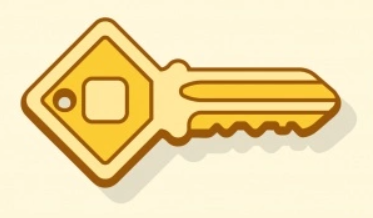
\includegraphics{key.png}
\end{figure}





\end{document}
